\chapter{Web Application}

\section{Overview}

To demonstrate the practical utility of the trained models in a real-world context, a full-stack web application named \textit{Gone Phishing} was developed. The application allows users to upload a \texttt{.eml} email file, which is then analyzed by the ensemble of fine-tuned transformer models to produce two complementary outputs: a spam/ham classification with confidence scores, and a multi-label emotion detection result characterising the psychological manipulation tactics present in the email.

The system is composed of two loosely coupled components: a \textbf{backend REST API} built with FastAPI that hosts the model inference pipeline, and a \textbf{frontend single-page application} implemented in vanilla HTML, CSS, and JavaScript that provides an interactive user interface. The backend is deployed as a Hugging Face Space (\texttt{Dpedrinho01/api-host}), while the frontend is served as a static site that communicates with the hosted API. A companion \textbf{Chrome browser extension} extends the same functionality directly into Gmail and Outlook Web, allowing users to scan emails without leaving their inbox.

\section{Application Architecture}

Figure~\ref{fig:webapp_architecture} illustrates the high-level architecture of the system. The user interacts exclusively with the browser-based frontend, which encodes the uploaded \texttt{.eml} file in Base64 and submits it to the \texttt{/predict/eml} endpoint of the FastAPI backend. The backend parses the raw email, extracts its textual content, and routes it through the spam detection ensemble and the emotion detection ensemble in sequence, returning a unified JSON response that the frontend renders as animated visual components.

\begin{figure}[ht]
    \centering
    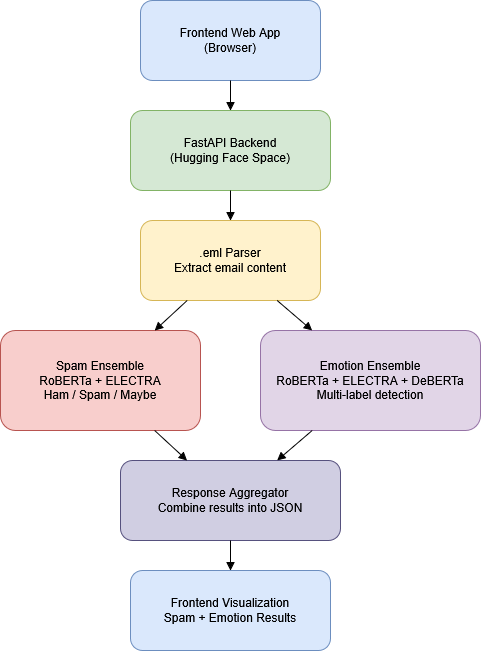
\includegraphics[width=0.85\textwidth]{figs/webapp_architecture.png}
    \caption{High-level architecture of the Gone Phishing web application. The browser-based frontend communicates with the FastAPI backend over HTTPS, which orchestrates inference across four transformer models.}
    \label{fig:webapp_architecture}
\end{figure}

\subsection{Backend API}

The backend is implemented in \texttt{api.py} using FastAPI and exposes a set of REST endpoints for spam and emotion classification. All cross-origin requests are permitted via \texttt{CORSMiddleware} to allow the decoupled frontend to communicate freely with the hosted service.

\subsubsection{Model Loading}

On application startup, four transformer model bundles are loaded from the Hugging Face Hub and moved to the available compute device (GPU if present, otherwise CPU):

\begin{itemize}
    \item \textbf{SpamModelBundle} — wraps a binary sequence classifier (either \acs{RoBERTa}-Large or \acs{ELECTRA}-Large) and reads its calibrated decision threshold from an accompanying \texttt{threshold\_config.json} file stored alongside the model checkpoint. The \texttt{predict\_proba} method tokenises the input text, runs a forward pass, and returns $P(\text{spam})$ via softmax.

    \item \textbf{EmotionModelBundle} — wraps a multi-label sequence classifier (\acs{RoBERTa}-Large or \acs{ELECTRA}-Large) and reads the per-class decision thresholds from a \texttt{model\_config.json} file. The \texttt{predict\_proba} method applies the sigmoid function to the raw logits and returns a dictionary mapping each of the eight consolidated emotion classes to a probability in $[0, 1]$.
\end{itemize}

All model inference is performed within \texttt{torch.no\_grad()} context managers to suppress gradient computation and reduce memory overhead during serving.

\subsubsection{EML Parsing}

The \texttt{extract\_text\_from\_eml} function uses Python's standard \texttt{email} library to parse raw \texttt{.eml} bytes into a structured message object. The function extracts the \texttt{Subject} and \texttt{From} header fields, then iterates over the message parts to collect \texttt{text/plain} content (preferred) or \texttt{text/html} content as a fallback. HTML content is stripped of tags using a regular expression and decoded with \texttt{html.unescape} before being concatenated into the final input string. Files exceeding 5\,MB are rejected at the API boundary.

\subsubsection{Ensemble Inference Logic}

\begin{itemize}
    \item \textbf{Spam ensemble.} The spam detection pipeline averages the softmax probabilities returned by the \acs{RoBERTa}-Large and \acs{ELECTRA}-Large spam classifiers. The averaged probability is compared against the mean of the two models' individual calibrated thresholds to produce the three-tier classification described in Chapter~4: \textit{ham} (below threshold), \textit{maybe spam} (at or above threshold but below 0.50), and \textit{spam} (at or above 0.50). This tiered scheme allows the interface to surface borderline cases to the user rather than forcing a hard binary decision.

    \item \textbf{Emotion ensemble.} The emotion detection pipeline obtains per-class probability vectors from both emotion models (\acs{RoBERTa}-Large and \acs{ELECTRA}-Large) and computes their element-wise arithmetic mean. Each averaged probability is then compared against the per-class threshold derived from the \acs{RoBERTa}-Large model's validation-set optimisation to determine whether a given emotion is detected. The \texttt{ensemble\_emotions} helper function returns both the list of detected emotion labels and a full list of \texttt{EmotionScore} objects sorted by probability in descending order.
\end{itemize}

\subsubsection{API Endpoints}

Table~\ref{tab:api_endpoints} summarises the endpoints exposed by the backend.

\begin{table}[htbp]
\centering
\caption{REST API endpoints exposed by the Gone Phishing backend.}
\label{tab:api_endpoints}
\begin{tabular}{llp{6.5cm}}
\hline
\textbf{Method} & \textbf{Path} & \textbf{Description} \\
\hline
GET  & \texttt{/}                & Root liveness check; returns service status message. \\
GET  & \texttt{/health}          & Returns device information and model load status for all four bundles. \\
POST & \texttt{/predict}         & Binary spam classification on raw text input. Supports single-model and ensemble modes. \\
POST & \texttt{/predict/emotion} & Multi-label emotion detection on raw text input; returns per-class scores for both emotion models and their ensemble average. \\
POST & \texttt{/predict/eml}     & Full pipeline analysis from a Base64-encoded \texttt{.eml} file. Parses the email, runs spam detection and emotion analysis, and returns a combined response. \\
POST & \texttt{/predict/batch}   & Batch spam classification for up to 50 text inputs. \\
\hline
\end{tabular}
\end{table}

The \texttt{/predict/eml} endpoint is the primary entry point used by the web frontend. It accepts a JSON body containing the filename and Base64-encoded file content, validates the file extension and size, extracts the email text, and returns a \texttt{FullEmlResponse} object combining the \texttt{PredictResponse} (spam result) and \texttt{EmotionPredictResponse} (emotion result).

\section{Chrome Browser Extension}

In addition to the web frontend, a companion Chrome extension named \textit{Gone Phishing} was developed to bring the same analysis capability directly into the user's inbox. The extension targets Gmail (\texttt{mail.google.com}) and Outlook Web (\texttt{outlook.live.com}, \texttt{outlook.office.com}), the two most widely used browser-based email clients.

\subsection{Architecture and Integration}

The extension is implemented as a Manifest V3 (MV3) package, consisting of a popup UI (\texttt{popup.html}, \texttt{popup.css}, \texttt{popup.js}) and a minimal content script that serves as a reference extraction helper. The popup handles all logic directly: when the user clicks the toolbar icon and presses \textit{Scan email}, the popup injects a one-off extraction function into the active tab via the \texttt{chrome.scripting.executeScript} API.

The injected function detects the active email client and extracts the email's subject, sender address, and body from the live DOM. For Gmail it targets the \texttt{.adn.ads} message containers and the \texttt{.a3s.aiL} body element; for Outlook Web it targets the \texttt{[data-testid="message-body"]} selector, with fallbacks for both clients. The extracted text is returned to the popup, which then calls the hosted API directly.

\subsection{API Usage}

Unlike the web frontend, which submits raw \texttt{.eml} files to the combined \texttt{/predict/eml} endpoint, the extension calls two endpoints separately:

\begin{itemize}
    \item \texttt{POST /predict} — for spam/ham ensemble classification, using \texttt{model: "ensemble"}.
    \item \texttt{POST /predict/emotion} — for multi-label emotion detection.
\end{itemize}

This approach avoids the overhead of Base64 encoding an \texttt{.eml} file, since the extension works with text already extracted from the rendered DOM rather than raw email files.

\subsection{User Interface}

The extension popup mirrors the visual design of the main web application, sharing the same dark aesthetic, typography, and animated probability bars. Spam results are displayed with the same three-tier verdict (ham, maybe spam, spam) and per-model breakdowns for both \acs{RoBERTa}-Large and \acs{ELECTRA}-Large. Detected emotions are shown as labelled chips with a bar chart of per-class probabilities. If no email is open in the active tab, the popup displays an idle state prompting the user to open an email before scanning.

\section{Deployment}

The backend API is hosted as a Hugging Face Space using a Docker runtime, which handles dependency installation from \texttt{requirements.txt} and launches the FastAPI application with Uvicorn. The four model checkpoints are downloaded from the Hugging Face Hub at startup via the \texttt{huggingface\_hub} library and cached within the Space container. The web frontend is served as a static site and communicates with the hosted API endpoint at \texttt{https://dpedrinho01-api-host.hf.space}. The Chrome extension points to the same hosted endpoint and requires no additional infrastructure.